

%%----------------------------------------%%
\begin{frame}[ctb!]
  \frametitle{Repository Components}
\footnotesize{
  \begin{figure}[htbp!]
  \begin{center}
    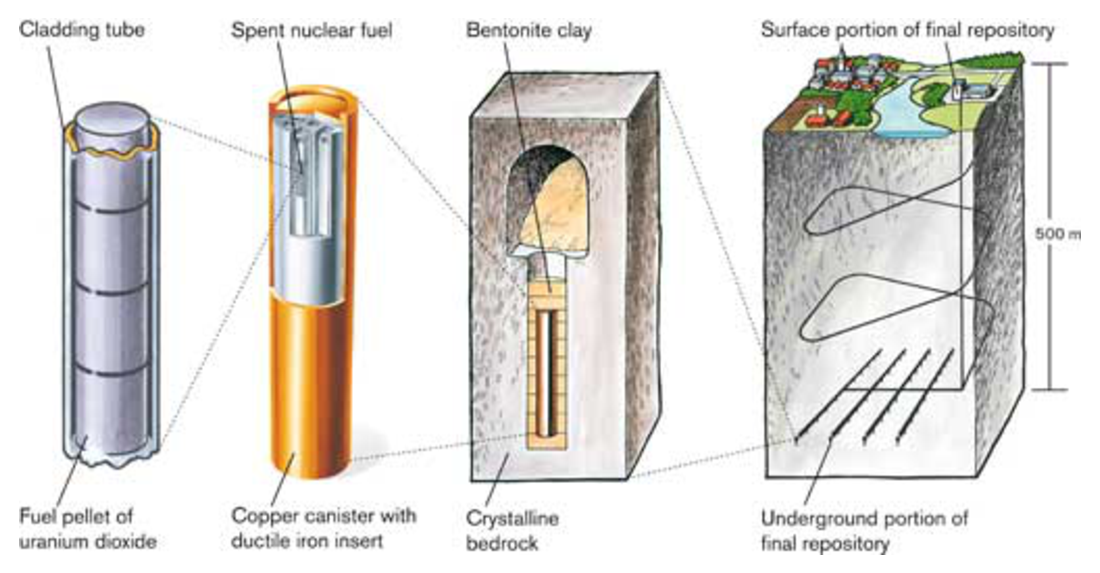
\includegraphics[width=0.7\textwidth]{./images/skb_components.eps}
  \end{center}
  \caption{Geologic disposal systems typically employ engineered barrier 
    systems as well as natural barrier systems. This is a Swedish concept in 
    granite \cite{ab_long-term_2006}.}
  \label{fig:skb_components}
\end{figure}

}
\end{frame}

%%----------------------------------------%%
\begin{frame}[ctb!]
  \frametitle{Engineered Barriers : Waste Forms}
\footnotesize{
  The first line of defense is the waste form.
  \begin{figure}[htbp!]
  \begin{center}
    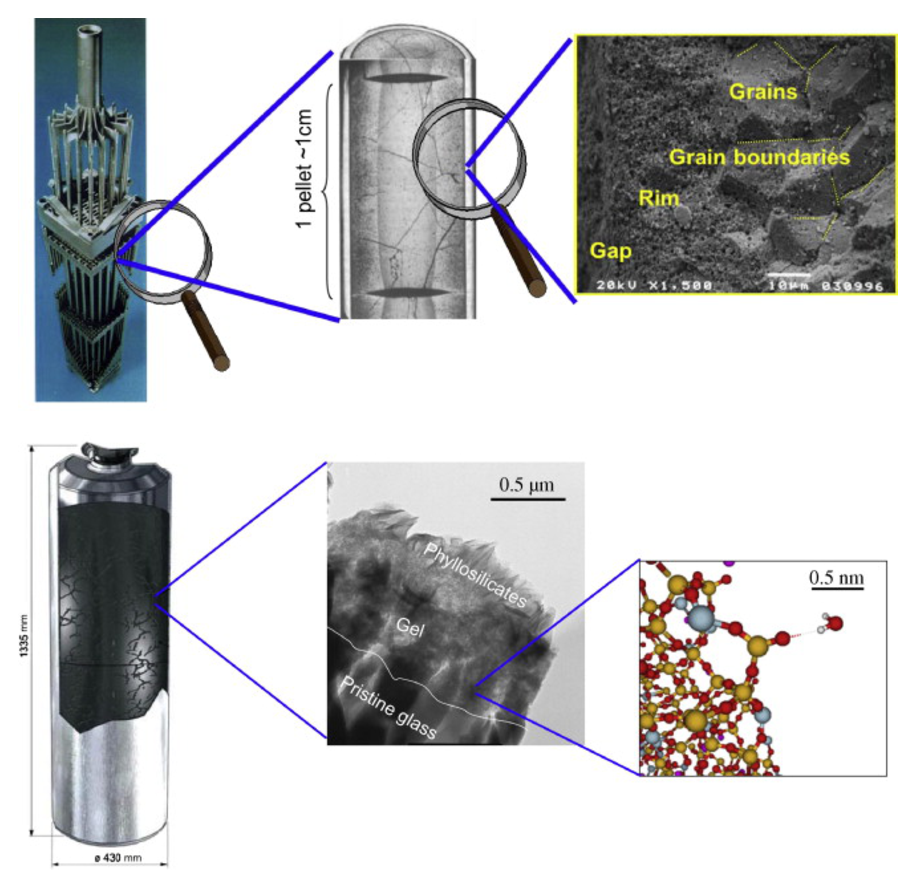
\includegraphics[width=0.5\textwidth]{./images/waste_forms_poinssot.eps}
  \end{center}
  \caption{A comparison of uranium oxide and borosilicate glass waste forms 
  \cite{poinssot_long-term_2012}.}
  \label{fig:waste_forms_poinssot}
\end{figure}

}
\end{frame}

%%----------------------------------------%%
\begin{frame}[ctb!]
  \frametitle{Engineered Barriers : Waste Packages}
\footnotesize{
  \begin{figure}[htbp!]
  \begin{center}
    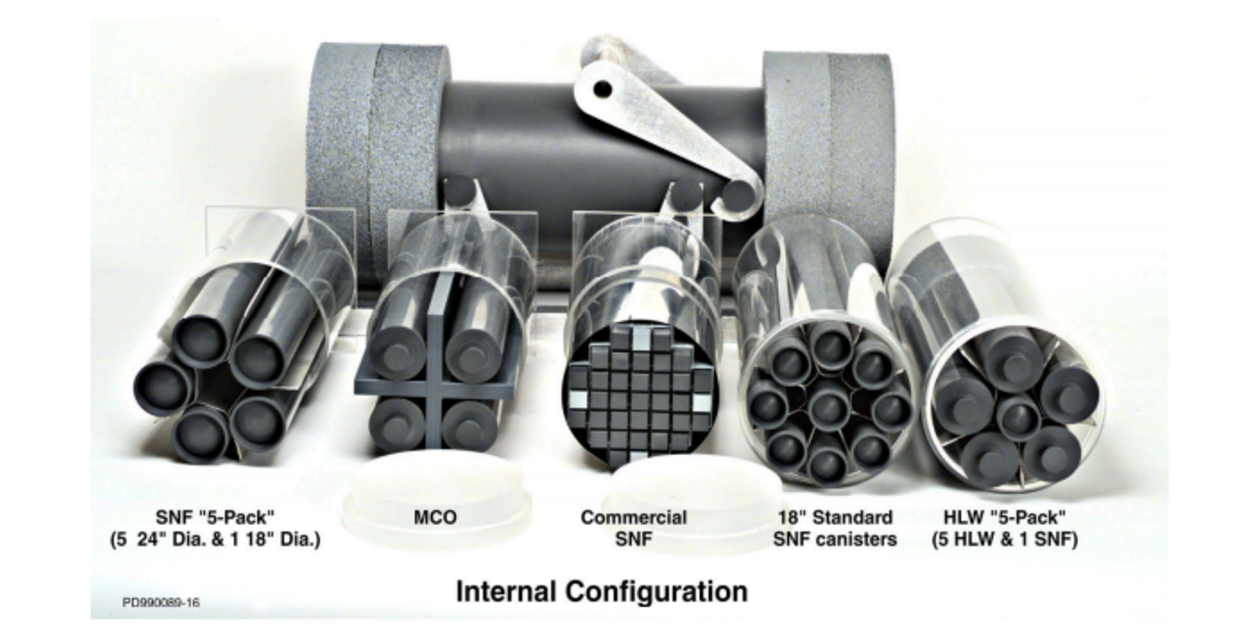
\includegraphics[width=0.7\textwidth]{./images/packages_ineel.eps}
  \end{center}
  \caption{Conceptual mockup of waste packages around waste forms 
    \cite{bridges_standardized_2001}.}
  \label{fig:packages}
\end{figure}

}
\end{frame}

%%----------------------------------------%%
\begin{frame}[ctb!]
  \frametitle{Engineered Barriers : Disposal Cask}
\footnotesize{
  \begin{figure}[htbp!]
  \begin{center}
    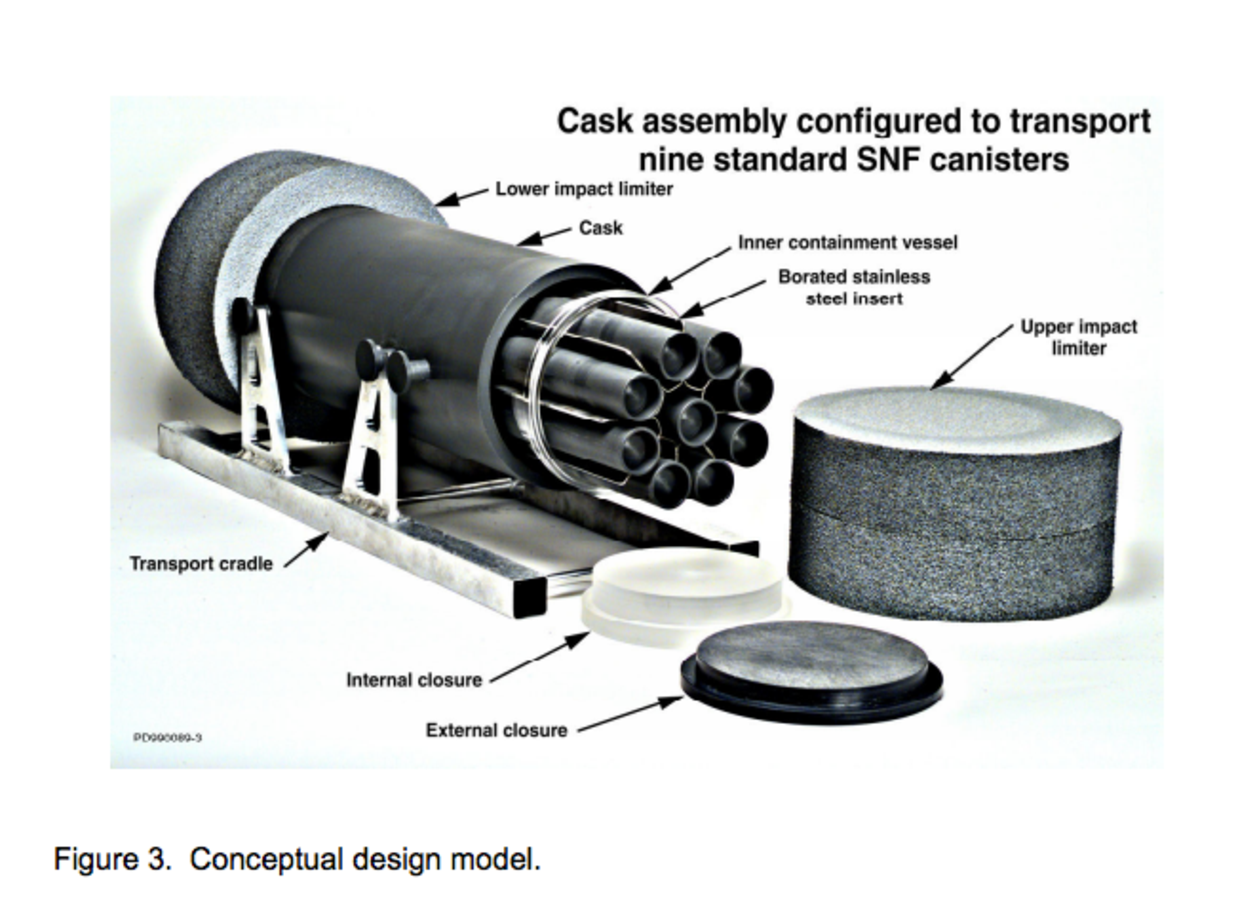
\includegraphics[width=0.7\textwidth]{./images/cask_ineel.eps}
  \end{center}
  \caption{Conceptual mockup of a transport and disposal cask 
    \cite{bridges_standardized_2001}.}
  \label{fig:packages}
\end{figure}

}
\end{frame}

%%----------------------------------------%%
\begin{frame}[ctb!]
  \frametitle{Engineered Barriers : Buffer}
\footnotesize{
  \begin{figure}[h!]
    \begin{center}
      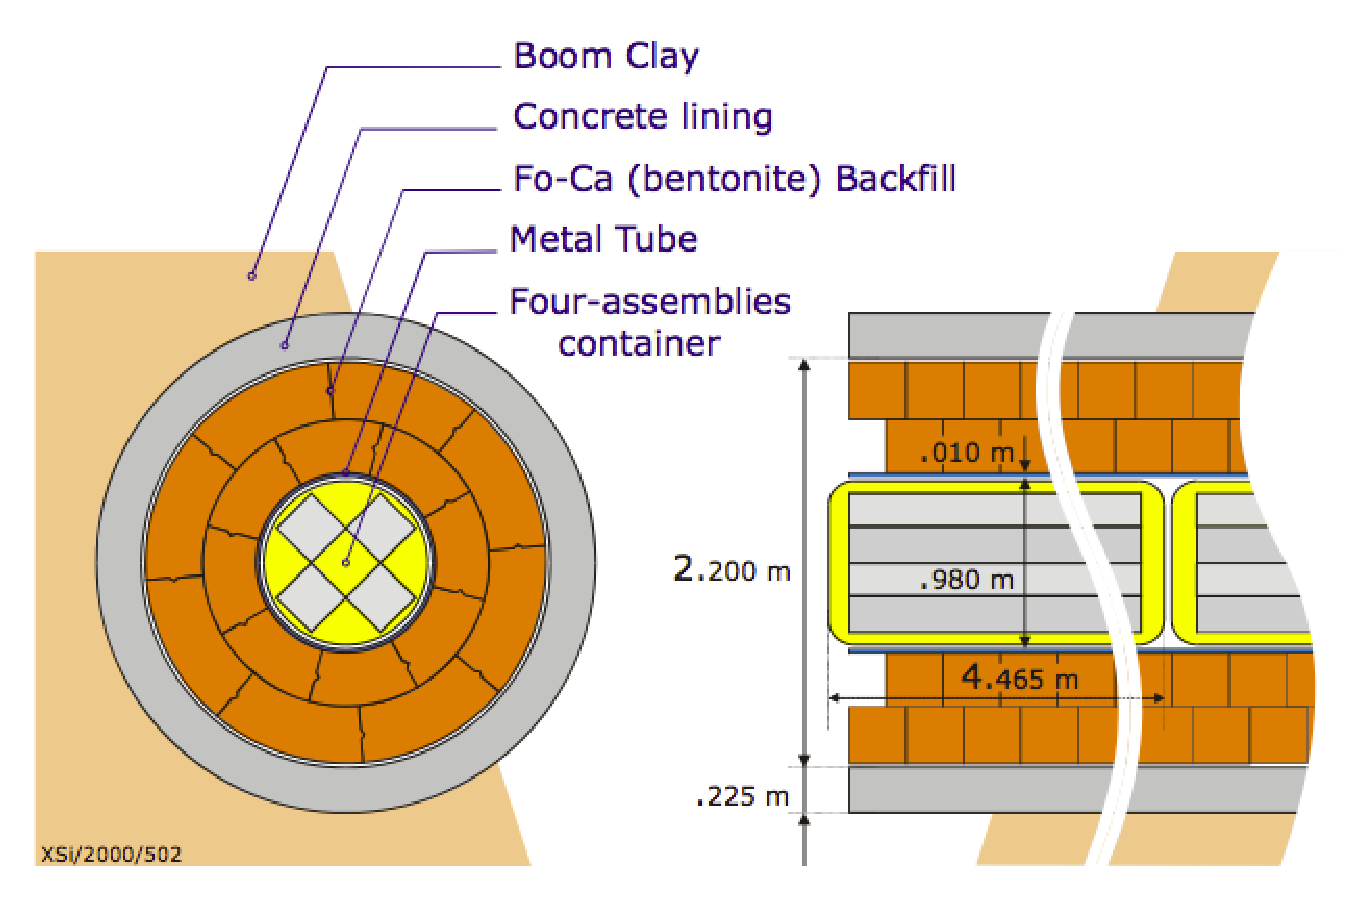
\includegraphics[height=.7\textheight]{./images/belgianClayRedImp.eps}
    \end{center}
    \caption{Belgian reference concept in Boom Clay 
    \cite{von_lensa_red-impact_2008}.}
    \label{fig:belgianClayRedImp}
  \end{figure}
}
\end{frame}

%%----------------------------------------%%
\begin{frame}[ctb!]
  \frametitle{Natural Barrier : Geology}
\footnotesize{
  \begin{figure}[htbp!]
  \begin{center}
    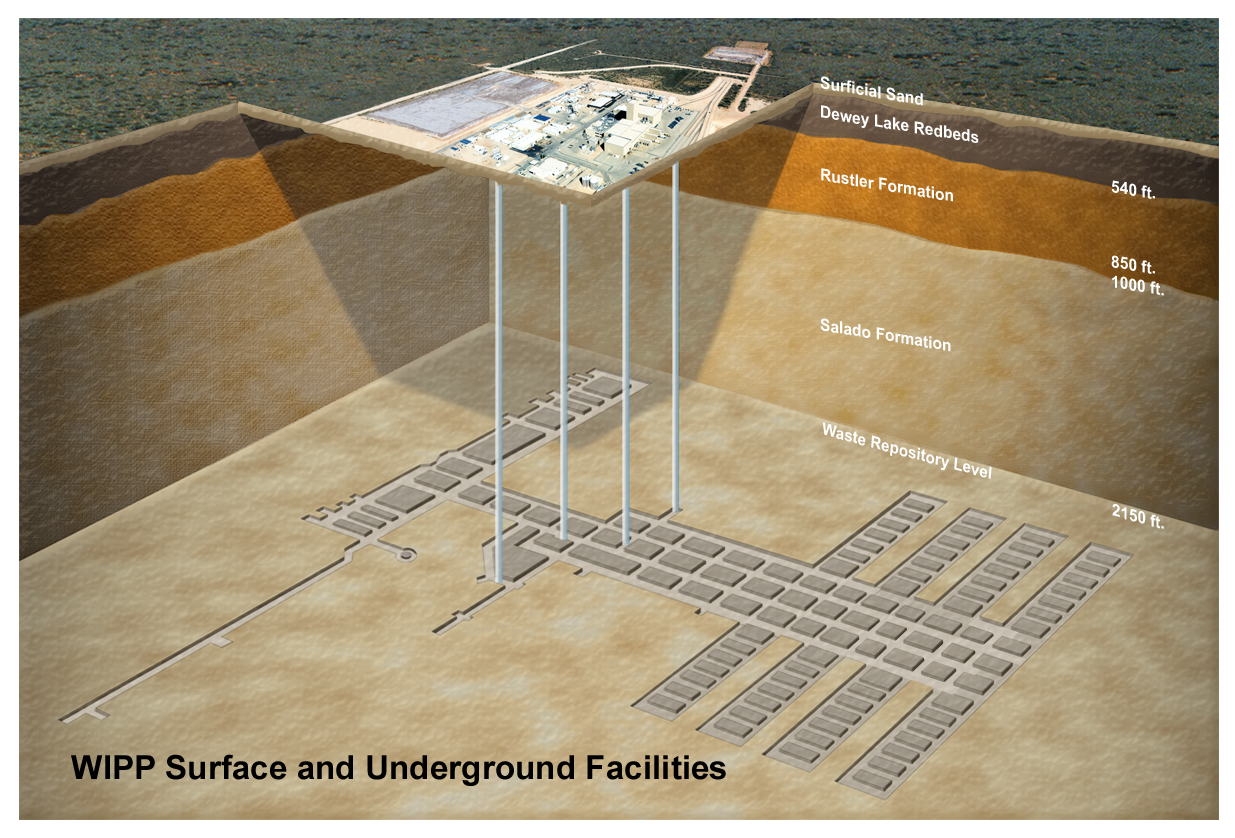
\includegraphics[width=0.7\textwidth]{./images/wipp_stratigraph.eps}
  \end{center}
  \caption{The Waste Isolation Pilot Plant has many geologic layers above the 
    salt bed \cite{doe_wipp_2013}.}
  \label{fig:wipp}
\end{figure}

}
\end{frame}
